\documentclass{beamer}

\usepackage{ucs}
\usepackage{amsfonts,amsmath}
\usepackage[utf8x]{inputenc}
\usepackage[protrusion=true,expansion=true]{microtype}
\usepackage{setspace}
\usepackage{pdfsync}
\usepackage{tikz}
\usepackage{macros}
\usepackage{mathpartir}
\usepackage{ulem}

\usetikzlibrary{automata, positioning, shapes.geometric, shapes.misc,
  chains, backgrounds, fit, decorations.pathmorphing}

\tikzset{
  state/.style={
    rounded rectangle,
    very thick,draw=black!50,
    top color=white, bottom color=black!20,
    minimum size=2em,
    text height=1.5ex,text depth=.25ex
  }
}

\tikzset{
  tribox/.style={
    isosceles triangle,
    isosceles triangle apex angle=40,
  }
}

\setbeamertemplate{footline}[frame number]
\setbeamertemplate{navigation symbols}{}
\setbeamertemplate{itemize item}[circle]

\usefonttheme{serif}
\usecolortheme[rgb={0.7,0.2,0.2}]{structure}
\definecolor{greenish}{rgb}{0.20,0.48,0.09} % vert des exemples


\date{\small June 20, 2012\\[0.5em]
  \scriptsize PPS -- Groupe de travail théorie des types et
  réalisabilité
}

\title{Certificates for incremental type checking}

\author[Matthias Puech \& Yann Régis-Gianas] {
  Matthias Puech\inst{1,2} \and Yann Régis-Gianas\inst{2}
}

\institute {
  \inst 1 {Dept. of Computer Science, University of Bologna} \and
  \inst 2 {Univ. Paris Diderot, Sorbonne Paris Cité, PPS, CNRS,  ${\pi}r^2$, INRIA}
}

\AtBeginSection[]
{\begin{frame}<beamer>
    \tableofcontents[currentsection]
  \end{frame}
}

\begin{document}

\frame\titlepage

\section{Introduction}
%
\section{Introduction}

\begin{frame}{A compiler designer's job}
  \begin{center}
    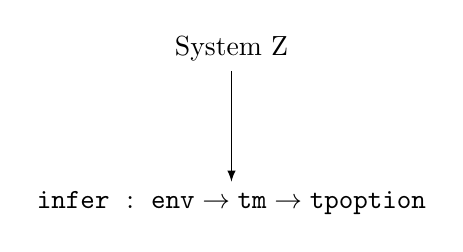
\begin{tikzpicture}[auto, >=latex]
      \node (ts) {System \sysname{Z}};

      \node (tc) [below=4em of ts] {$\tt \fct{infer}\ :\ \cst{env} \to \cst{tm} \to \app
        {\cst{tp}} \cst{option}$};

      \path[->] (ts) edge (tc);
    \end{tikzpicture}

    \vspace{2em}
    set of declarative inference rules $\to$ decision algorithm
  \end{center}
  \pause
  \begin{itemize}
  \item non trivial (inference, conversion\ldots)
  \item non compositional
  \end{itemize}

\end{frame}

\begin{frame}{\textcolor{greenish}{Example:} System \sysname{T}$_{<:}$}
  \begin{block}{Syntax}
    \vspace{-2em}
    \begin{align*}
      M &\gequal \z \gor \s M \gor M M \gor \lam x M \gor
      \recb M N x y P \\
      A &\gequal \nat \gor \even \gor \odd \gor A \to A
    \end{align*}
  \end{block}
  \begin{block}{Typing rules}
    \vspace{-2em}
    \begin{mathpar}
      \infer{\jts M \nat \and \jts N A \and \infer*{}{\mbox{$
            \begin{array}{c}
              [\jts {\var x} \nat] \quad
              [\jts {\var y} A] \\[-0.3em]
              \vdots\\
              \jts P A
            \end{array}
            $}} }{\jts {\recb M N x y P} A}

      \only<2>\alert{\infer{\jts M A \and \jsub A B}{\jts M B}}

    \end{mathpar}
  \end{block}
  \pause
  \begin{center}
    {\large\it \alert{Not syntax directed!}}
  \end{center}
\end{frame}

\begin{frame}{\textcolor{greenish}{Example:} System \sysname{T}$_{<:}$}
  \begin{block}{Typing algorithm}
    \begin{overlayarea}\textwidth{8em}
      \large \only<1>{$$ \infer{\Gamma\jts M {A\to B} \and \Gamma\jts
          N A}{\Gamma\jts{\app M N} B}
    $$}

  \only<2>{$$ \infer{ \Gamma\jts M {A\to B} \and \infer*{ \Gamma\jts N
        {A'} \and \Gamma\jsub {A'} A }{ \Gamma\jts N A } }{
      \Gamma\jts{\app M N} B }
    $$}

  \only<3>{$$ \infer{ \Gamma\jts M \nat \and \Gamma\jts N A \and
      \Gamma, \var x :\nat, \var y: A\jts P A }{\jts {\recb M N x y P}
      A}
    $$}

  \only<4->{$$ \infer{ \Gamma\jts M {T_M} \and \Gamma\jsub{T_M}{\nat}
      \and \Gamma\jts N T_N
      \\
      \Gamma, \var x:\nat, \var y:T_N\jts P {T_P}
      \\
      \Gamma, \var x:\nat, \var y:T_N\sqcap T_P\jts P {T_N\sqcap T_P}
    }{ \Gamma\jts {\recb M N x y P} {T_N\sqcap T_P} }
    $$}

  \only<5>{
    \begin{itemize}
    \item Far from the declarative system
    \item Hard to prove
    \end{itemize}
  }
\end{overlayarea}
  \end{block}
\end{frame}

\begin{frame}{How to trust your typing algorithm?}
  \begin{block}{Option 1}
    Prove equivalence:
    $$
    \app{\fct{infer}}\app{\Gamma}{M}=\app{\cst{Some}} A
    \quad\text{iff}\quad
    \vdash M : A
    $$
  \end{block}
  \pause
  \begin{block}{Option 2}
    Return a System \sysname{T}$_{<:}$ derivation:
    $$
    \fct{infer}\ :\ \cst{env}\to\cst{tm}\to\cst{tp}\times\cst{deriv}
    $$
  \end{block}
\end{frame}

%%% Local Variables: 
%%% mode: latex
%%% TeX-master: "slides"
%%% End: 

\frame\tableofcontents
\section{Using \sysname{Gasp}}
\subsection{As a programmer}

\begin{frame}{\textcolor{greenish}{Example}}

  {\tt\qquad Gasp 0.1} \\[1em]

  \theprompt
  \pause
  $
  \finfer{(\recb{\s\z}{\s\z} x y {\s {\var x}})}
  $
  \\[1em]
  \pause
  $\small
  \begin{aligned}
    \md_1\ &:\ \ \vdash \s\z : \odd = \infer{\infer{ }{\vdash\z:\even}}{\vdash\s\z : \odd}\\
    \pause
    \md_2[{{\vdash x :\nat}} ]\ &: \ \ \vdash \s{\var x} : \nat =
    \infer{[\vdash x : \nat]}{\vdash \s{\var x} : \nat}\\
    \pause
    \md_3\ &:\ \ \vdash \s\z : \nat = \infer{\md_1\and \infer*{ }{\vdash
      \odd\leq\nat}}{\vdash\s\z:\nat}
    \\
    \pause
    \fbox{$\md_4$}\ &:\ \ \vdash \recb{\s\z}{\s\z} x y {\s {\var x}} :
    \nat = \infer{\md_1\and\md_3\and\infer*{[\vdash \var x:\nat]}{\md_2}}{\vdash \recb{\s\z}{\s\z} x y {\s {\var x}} :
    \nat}
  \end{aligned}
  $

  \vfill\pause
    \begin{block}{Functions}
      $\finfer{M}$ : derivation generator \\
    \end{block}
\end{frame}

\begin{frame}{\textcolor{greenish}{Example}}

  \theprompt
  \only<1>{$\finfer{(\recb{\s{\s\z}}{{\s\z}} x y {{\s {\var x}}})}$}%
  \only<2>{$\finfer{(\recb{\s{\alert{\s\z}}}{\alert{\s\z}} x y {\alert{\s {\var x}}})}$}%
  \only<3>{$\finfer{(\recb{\s{\md_1}}{\md_3} x y {\alert{\s {\var x}}})}$}%
  \only<4>{$\finfer{(\recb{\s{\fget\md_1}}{\fget\md_3} x y {\alert{\s {\var x}}})}$}%
  \only<5>{$\finfer{(\recb{\s{\fget\md_1}}{\fget\md_3} x y {\fget{\md_2}})}$}%
  \only<6->{$\finfer{(\recb{\s{\fget\md_1}}{\fget\md_3} x y {\fget{\md_2[\finfer{x}]}})}$}%

  \begin{visibleenv}<7->
    \begin{align*}
      \ldots &\ \text{(all of the above, plus:)}\\
      \md_5\ &:\ \vdash \s{\s\z}:\nat = \ldots \\
      \fbox{$\md_6$}\ &:\ \vdash \recb{\s{\s\z}}{\s\z} x y {\s{\var x}}:\nat = \ldots
    \end{align*}
  \end{visibleenv}
  \only<8->{\theprompt$\finfer{(\recb{\fget{\md_5}}{\fget{\md_3}}xy{\fget{\md_2[\md_2[\finfer{x}]]}})}$}%
  \vfill
    \begin{block}{Functions}
      $\finfer{M}$ : derivation generator \\
      \visible<4->{$\fget{\md}$ : coercion from derivation to the program it types}
    \end{block}

\end{frame}

\begin{frame}{Methodology}
  \begin{itemize}
  \item user inputs commands made of terms (programs), functions
    ($\finfer{}$, $\fget{}$) and \emph{contextual metavariables} $\md_i$
  \item to each function $A\to B$ there is an ``inverse'' $B\to A$
    (put output back into input)
  \item system evaluates functions to value (derivations)
  \item checks value (kernel)
  \item extracts (from context) and names all subterms to a map
    (repository) for future reuse: \emph{slicing}
  \end{itemize}
\end{frame}

\subsection{The \LF\ notation for derivations}

\begin{frame}{What notation for derivations?}
  % TODO
\end{frame}

\subsection{As a type system designer}

\begin{frame}{How to write the unsafe type checker?}
  The computation language \CL:
  \begin{itemize}
  \item an unsafe language to manipulate \LF\ objects
  \item but with runtime check: each input \& output must be well-typed
  \end{itemize}
\end{frame}

\begin{frame}{\textcolor{greenish}{Example}}
  \begin{onlyenv}<1-3>
    \begin{mathleft}
      \finfer{}\ :\ \prd M {\cst{tm}} \sig A {\cst{tp}} (\vdash M : A)
      =
      \\
      \pause
      \lamd M \match{M} \\
      \pause
      \quad\caseb{\z} \pair {\cst{even}}{\infer{ }{\vdash \cst o : \cst{even}}} \\
      \quad\caseb{\s M}
      \match{\finfer M} \\
      \quad\quad\caseb{\pair{\cst{even}}\md}
      \pair {\cst{odd}}{\infer\md{\vdash\app{\cst{s}} M : \cst{odd}}} \\
      \quad\quad\caseb{\pair{\cst{odd}}\md}
      \pair {\cst{even}}{\infer\md{\vdash\app{\cst{s}} M : \cst{even}}} \\
      \quad\quad\caseb{\pair{\cst{nat}}\md}
      \pair {\cst{nat}}{\infer\md{\vdash\app{\cst{s}} M : \cst{nat}}} \\
    \end{mathleft}
  \end{onlyenv}

  \begin{onlyenv}<4>
    \begin{mathleft}
  \quad\caseb{\app{M}N} \\
  \quad\quad\letd {\pair {A_1\to B} {\md_1}} {\finfer{M}} \\
  \quad\quad\letd {\pair {A_2} {\md_2}} {\finfer{N}} \\
  \quad\quad\letd {\md_{\leq}} {\fleq {A_1} {A_2}} \\
  \quad\quad
  \match{\md_{\leq}} \\
  \quad\quad\quad\caseb{\infer{ }{\vdash A\leq A}}
  \pair {B} {\infer{\md_1 \and \md_2}{\vdash \app M N : B}} \\
  \quad\quad\quad\caseb{\_}
  \pair {B} {\infer{\md_1 \and \infer*{\md_2 \and \md_{\leq}}{\vdash N
      : A_1}}{\vdash \app M N : B}}
    \end{mathleft}

    \begin{block}{Functions}
      $\fleq{}{}\ :\ \prd A
      {\cst{tp}} \prd B {\cst{tp}} \vdash A\leq B = \ldots$
    \end{block}
  \end{onlyenv}

  % lambda
  \begin{onlyenv}<5-8>
    \begin{mathleft}
      \quad\caseb{\tlam x A M}
      \uncover<6->{
        \\\quad\quad
        \syntax{let}{\pair B \md}
        \only<8->{\syntax{in}{\env {$\md_{\var x}$}{(\vdash {\var x} : A)}}}
        \syntax{=}
        \\\quad\quad\quad
        {\finfer {\alt<-6> M {\gsubst M {\msubst x {\fget{\pair A {\md_{\var
                      x}}}}}}}}
        \syntax{in}
        \\\quad\quad
        \pair {A\to B}
        {\infer{
            \mbox{$      \begin{array}{c}
                \uncover<7->{{[\md_{\var x}]} \\}
                {\md}
              \end{array}
              $}    }{
            \vdash\lam x M : A\to B
          }}
      }      \\[2em]
      \quad\text{\only<7->\sout{$\caseb{\var x}\ \uncover<6->{???}$}}
    \end{mathleft}
    \uncover<7->{
      \begin{block}{Note}
        $\finfer{\fget{\pair{A}{\md}}} = \pair{A}{\md}$
      \end{block}
    }
  \end{onlyenv}

  \begin{onlyenv}<9->
    \begin{mathleft}
  \quad\caseb{\recb M N x y P} \\
  \quad\quad
  \letd {\pair {A_M} {\md_M}} {\finfer{M}} \\
  \quad\quad
  \letd {\md_{A_M}} {{A_M} \leq \cst{nat}} \\
  \quad\quad
  \letd {\pair {A_N} {\md_N}} {\finfer{N}} \\
  \quad\quad
  \syntax{let} {\pair {A_P} {\md_P}} \syntax{in}
  {(\envcons {\env {$\md_x$} {(\vdash
        \var x : \cst{nat})}} {$\md_y$} {(\vdash\var y : A_N)})} = \\
  \quad\quad\quad
  {\finfer{\gsubst P {\msubstcons {\msubst x
          {\fget{\pair{\cst{nat}}{\md_x}}}} y
        {\fget{\pair{A_N}{\md_y}}}}}} \syntax{in}\\
  \quad\quad\letd {\pair A {\pair{\md_{A_N}}{\md_{A_P}}}} {{A_N} \sqcap {A_P}} \\
  \quad\quad
  \syntax{let} {\pair {\_} {\md_P}} \syntax{in}
  {(\envcons {\env {$\md_x$} {(\vdash
        \var x : \cst{nat})}} {$\md_y$} {(\vdash\var y : A)})} = \\
  \quad\quad\quad
  {\finfer{\gsubst P {\msubstcons {\msubst x
          {\fget{\pair{\cst{nat}}{\md_x}}}} y
        {\fget{\pair{A}{\md_y}}}}}} \syntax{in}\\
  \quad\quad\pair {A} {
    \infer{
      \infer*{\md_M \and \md_{A_M}}
      {\vdash M : A} \and
      \infer*{\md_N \and \md_{A_N}}
      {\vdash N : A}\and
      \infer*{\infer*{}{\mbox{$
        \begin{array}{c}
          [\md_x] [\md_y] \\
          \md_P
      \end{array}
        $}} \and \md_{A_P}}{\vdash P : A}
    }{
      \vdash \recb M N x y P : A
    }
  }
    \end{mathleft}
    \begin{block}{Functions}
      $\sqcap\ :\ \prd{A}{\cst{tp}} \prd{B}{\cst{tp}} \sig C {\cst{tp}}
      (\vdash A\leq C )\times(\vdash B\leq C) = \ldots$
    \end{block}
  \end{onlyenv}

\end{frame}

\begin{frame}{Discussion}
  \begin{itemize}[<+->]
  \item the ``type'' of a function is more of a \emph{contract}:
    \begin{figure}
      \centering
      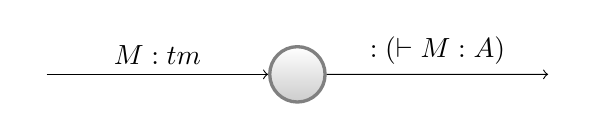
\begin{tikzpicture}[auto]
        \node (in) {}; \node (F) [state, right=8em of in] {$\finfer{}$};
        \node (out) [right=8em of F]{};

        \path[->] (in) edge node (m) {$M : \cst{tm}$} (F) (F) edge
        node (d)
        {$\md : (\vdash M : A)$} (out);
      \end{tikzpicture}
    \end{figure}
  \item ``inverses'' used to feed output back to input, same idea as
    \emph{context-free} typing:

    $$M \gequal \var x \gor \app M M \gor \tlam x A M \gor \{\var x :
    A\} $$
    \begin{mathpar}
      \infer{ \vdash \gsubst M {\msubst x {\{\var x:A\}}} : B }{ \vdash
        \tlam x A M : A\to B }

      \infer{ }{ \vdash \{\var x : A\} : A }
    \end{mathpar}

  \end{itemize}
  
\end{frame}

%%% Local Variables: 
%%% mode: latex
%%% TeX-master: "slides"
%%% End: 

%
\begin{frame}{Certifying procedures}
  What is a certifying procedure?

  \begin{figure}
    \centering
    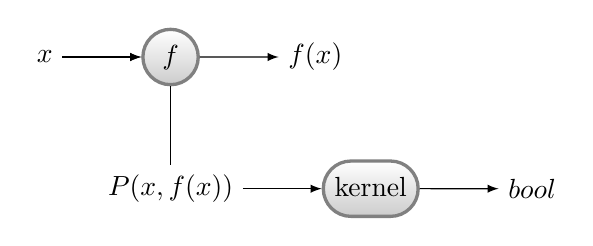
\begin{tikzpicture}[auto, >=latex]

      \node (input) {$x$};

      \node (F) [state, right=of input] {$\fct{f}$};

      \node (output) [right=of F]{$\fct{f}(x)$};

      \path[->] (input) edge (F) (F) edge (output);

      \pause

      \node (P) [below=of F]{$P(x, \fct{f}(x))$};

      \node (check) [state, right=of P] {kernel};

      \node (bool) [right=of check] {$\cst{bool}$};

      \path[->]

      (input) edge (F)

      (F) [-] edge (P)

      (P) [->] edge (check)

      (check) edge (bool)

      ;

    \end{tikzpicture}
  \end{figure}

  \begin{itemize}[<3->]
  \item untrusted, complex function
  \item generic and small kernel (dB principle)
  \end{itemize}

\end{frame}

\begin{frame}{Certifying procedures}
  \begin{examples}
    \begin{itemize}
    \begin{onlyenv}<1>
    \item Theorem proving
      \begin{figure}
        \centering
        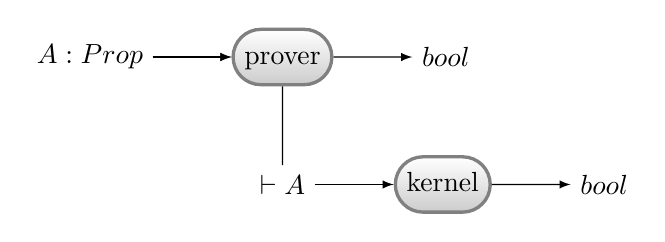
\begin{tikzpicture}[auto, >=latex]

          \node (input) {$A : \cst{Prop}$};

          \node (F) [state, right=of input] {prover};

          \node (output) [right=of F]{$\cst{bool}$};

          \path[->] (input) edge (F) (F) edge (output);

          \node (P) [below=of F]{$\vdash A$};

          \node (check) [state, right=of P] {kernel};

          \node (bool) [right=of check] {$\cst{bool}$};

          \path[->]

          (input) edge (F)

          (F) [-] edge (P)

          (P) [->] edge (check)

          (check) edge (bool)

          ;

        \end{tikzpicture}
      \end{figure}
    \end{onlyenv}
      \begin{onlyenv}<2>
      \item Proof-carrying code
      \begin{figure}
        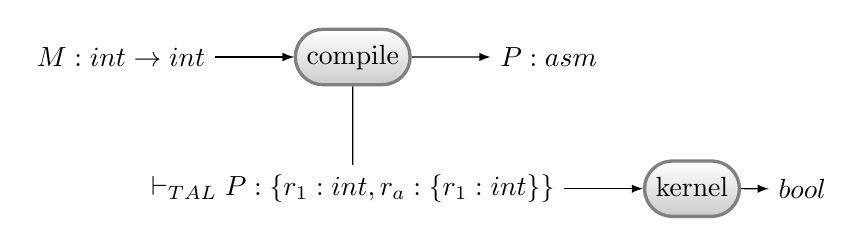
\begin{tikzpicture}[auto, >=latex]

          \node (input) {$M : \cst{int}\to\cst{int}$};

          \node (F) [state, right=of input] {compile};

          \node (output) [right=of F]{$P : \sysname{asm}$};

          \path[->] (input) edge (F) (F) edge (output);

          \node (P) [below=of F]{$\small\vdash_{\sysname{TAL}} P : \{r_1:\cst{int}, r_a:\{r_1:\cst{int}\}\}$};

          \node (check) [state, right=of P] {kernel};

          \node (bool) [right=1em of check] {$\cst{bool}$};

          \path[->]

          (input) edge (F)

          (F) [-] edge (P)

          (P) [->] edge (check)

          (check) edge (bool)

          ;

        \end{tikzpicture}
\\[2em]
{\footnotesize To call $P$, the caller must place an integer in $r_1$ and a
        return label in $r_a$, the return label must accept an integer
        in $r_1$.
}      \end{figure}
    \end{onlyenv}
    \begin{onlyenv}<3>
    \item \sysname{LCF} Tactics
      \begin{figure}
        \centering
        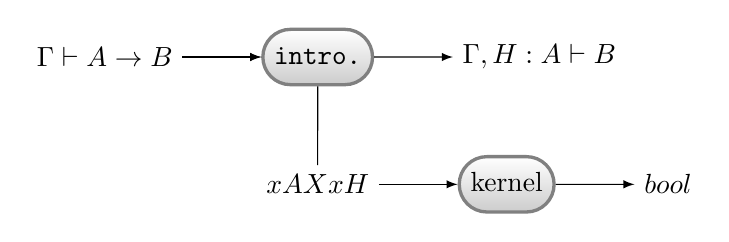
\begin{tikzpicture}[auto, >=latex]

          \node (input) {$\Gamma\vdash A\to B$};

          \node (F) [state, right=of input] {\tt intro.};

          \node (output) [right=of F]{$\Gamma, H:A\vdash B$};

          \path[->] (input) edge (F) (F) edge (output);

          \node (P) [below=of F]{$\tlam x A \smeta X {\msubst x H}$};

          \node (check) [state, right=of P] {kernel};

          \node (bool) [right=of check] {$\cst{bool}$};

          \path[->]

          (input) edge (F)

          (F) [-] edge (P)

          (P) [->] edge (check)

          (check) edge (bool)

          ;

        \end{tikzpicture}
      \end{figure}
    \end{onlyenv}
    \begin{onlyenv}<4>
    \item Type checking
      \begin{figure}
        \centering
        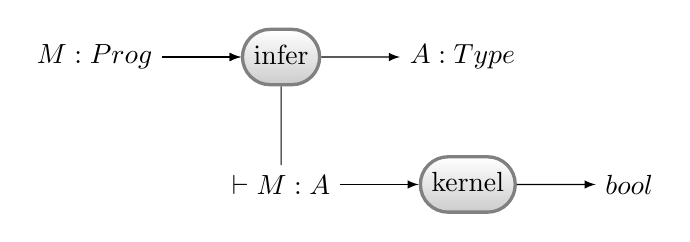
\begin{tikzpicture}[auto, >=latex]

          \node (input) {$M : \cst{Prog}$};

          \node (F) [state, right=of input] {infer};

          \node (output) [right=of F]{$A : \cst{Type}$};

          \path[->] (input) edge (F) (F) edge (output);

          \node (P) [below=of F]{$\vdash M : A$};

          \node (check) [state, right=of P] {kernel};

          \node (bool) [right=of check] {$\cst{bool}$};

          \path[->]

          (input) edge (F)

          (F) [-] edge (P)

          (P) [->] edge (check)

          (check) edge (bool)

          ;

        \end{tikzpicture}
      \end{figure}
    \end{onlyenv}
    \end{itemize}
  \end{examples}
\end{frame}

\subsection{LF}

\subsection{Writing a type-checker}



%%% Local Variables: 
%%% mode: latex
%%% TeX-master: "slides"
%%% End: 

\section{The design of \sysname{Gasp}}
%
%%% Local Variables: 
%%% mode: latex
%%% TeX-master: "slides"
%%% End: 



\end{document}
